
\chapter{概率}
\label{chap:probability}

\section{基本问题}
\label{sec:basic-probability-problems}

\begin{example}
  某个国家的人们都仅想生养男孩,所有家庭在生养男孩之前是不会停止生养的。如果生养的是女孩,他们将继续生养,只到生个男孩为止。如果生养的是男孩,他们将不再生养。那么,在这个国家男孩和女孩的比例是多少?
\end{example}
\begin{proof}[提示]
  举个例子,假如有16个家庭,按概率,大概有8个家庭头胎生男孩,8个家庭头胎生女孩。头胎生女孩的8个家庭又有4个二胎生男孩,4个二胎生女孩。4个二胎生女孩的家庭又有2个三胎生男孩,2个三胎生女孩。2个三胎生女孩的家庭又有1个四胎生男孩,1个四胎生女孩。1个四胎生女孩的家庭再继续下去,

  \begin{center}
    \begin{tikzpicture}[scale=.8]
      \node(N02)[draw,circle,pattern=dots]at(0,0){1};%\fill[color=white](0,0)circle(.2)node{1};
      \foreach \x/\v in{1/2, 2/4, 3/8, 4/16, 5/32, 6/64}{
        \node(N\x1)[draw,circle,fill=red!20]at(2*\x,1.5){\tiny $\frac1{\v}$};
        \node(N\x2)[draw,circle]at(2*\x,0){\tiny $\frac1{\v}$};
      }
      \node(N71)[draw,circle,fill=red!20]at(2*7,1.5){\tiny $\cdots$};
      \node(N72)[draw,circle]at(2*7,0){\tiny $\cdots$};
      \foreach \x/\y in{0/1,1/2,2/3,3/4,4/5,5/6,6/7}{
        \draw[->](N\x2)--(N\y1);
        \draw[->](N\x2)--(N\y2);
      }
    \end{tikzpicture}
  \end{center}
  图中阴影部分\tikz{\draw[fill=red!20](0,0)circle(.2)}表示生养了男孩,此家庭在此位置停止生养;\tikz{\draw(0,0)circle(.2)}表示此家庭在此位置生养了女孩,此家庭在此位置继续生养。

  这样无穷尽的下去,可以得到所有第一代家庭生养的男孩总数与女孩总数都为
  \begin{align*}
    16\times\left(\frac12 + \frac14 + \frac18 + \frac1{16}+\cdots\right)=16\times 1 = 16
  \end{align*}

  如果第一代家族总数是无数多的,那么比例会接近于$1:1$。而事实上,第二代家庭、第三代家庭等都是可以直接算到第一代家庭中来计算而不会影响概率的本身,而人类总是无穷无尽地在繁衍,所以家庭数可以当做是无限大的,该地的男孩女孩比例总会随着时间的流逝而越来越接近于$1:1$。
\end{proof}


\begin{example}
  在一线段上随机取两个点将线段分为三份,求此三份线段能组成一个三角形的概率是多少?
\end{example}
\begin{proof}[提示]
  转换为几何模型。不妨设线段的长度为1,记线段上随机取的两个点到同一个顶点的距离分别为$x$和$y$。由对称性,不妨只考虑$0<x<y<1$的情况。从而$x,y-x,1-y$三个长度的线段能组成三角形,等价于以下条件同时成立:
  \begin{align*}
    \begin{cases}
      x < (y-x) + (1-y)\\
      y - x < x + (1 - y)\\
      1 - y < x + (y - x)
    \end{cases}
    \implies
    \begin{cases}
      x<\frac12\\ y<x + \frac12\\ y>\frac12
    \end{cases}
  \end{align*}
  在笛卡尔坐标上作出上述图形,利用面积比可以容易得到概率。
  \begin{center}
    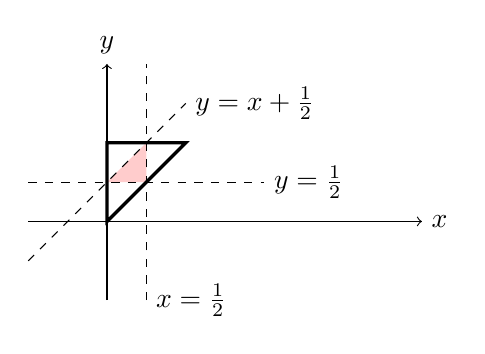
\begin{tikzpicture}[scale=1.0]
      \fill[color=red!20](0,.5)--(.5,.5)--(.5,1)--cycle;
      \draw[->](-1,0)--(4,0)node[right]{$x$};
      \draw[->](0,-1)--(0,2)node[above]{$y$};
      \draw[very thick](0,0)--(1,1)--(0,1)--cycle; % domain
      \draw[dashed](-1,-.5)--(-.5,0)--(.5,1)--(1,1.5)node[right]{$y=x+\frac12$};
      \draw[dashed](-1,.5)--(2,.5)node[right]{$y=\frac12$};
      \draw[dashed](.5,-1)node[right]{$x=\frac12$}--(.5,2);
    \end{tikzpicture}
  \end{center}
  可行区域是由$0<x<y<1$组成的粗边框三角形。图中阴影中的点对应的$(x,y)$为可以组成三角形的情况,从而其概率为$\frac14$。
\end{proof}

\begin{example}
  在一个圆周上随机取三个点,求此三点能组成一个锐角三角形的概率是多少?
\end{example}
\begin{proof}[提示]
  由对称性,可以考虑固定一个点的情况。过此固定点作圆的直径,那么三个点组成锐角三角形等价于三个点不能落在同一个半圆上。但这个条件有点不好用,需要考虑的分支有点多。不妨设另外两个动点对应的幅角为$x,y$,且由对称性,不妨假设$0<x< y<2\pi$。

  幅角分别为$0,x,y$(且$0<x<y<2\pi$)所对应的圆(不妨设为单位圆)上的三点组成的三角形,且三角形将圆分割成三段弧长分别为$x,(y-x),(2\pi-y)$的弧,从而三角形的三个内角分别为$x/2, (y-x)/2, \pi - y/2$。从而三角形是锐角三角形,等价于以下条件同时成立:
  \begin{align*}
    \begin{cases}
      x/2 < \pi/2\\ (y-x)/2 < \pi/2 \\ (2\pi - y)/2 < \pi/2
    \end{cases}
    \implies
    \begin{cases}
      x < \pi \\ y < x + \pi \\ y > \pi
    \end{cases}
  \end{align*}
  或者更直接的,由锐角三角形可知三条弧都要小于$\pi$,从而马上可得上面结论。

  \begin{center}
    \begin{tikzpicture}[scale=1.0]
      \begin{scope}[scale=2.0]
        \draw(0,0)circle(1);
        \coordinate[label=below right:\small 固定点](A)at(1,0);
        \coordinate[label=above right:\small 动点](B)at(50:1);
        \coordinate[label=below left:\small 动点](C)at(210:1);
        \tkzDrawPoints(A,B,C);
        \draw(A)--(B)--(C)--cycle;
        \draw[->](-1.3,0)--(1.4,0);
        \draw[->](0,-1.3)--(0,1.4);
        \foreach \r/\d in{1.2/10}{
          \foreach \x/\y/\v in{0/50/$x$,50/210/$y-x$,210/360/$2\pi-y$}{
            \draw[dashed,<->](\x+\d:\r)arc(\x+\d:\y-\d:\r)node[midway,sloped,fill=white]{\v};
          }
        }
      \end{scope}
      \begin{scope}[shift={(5.5,0)}]
        \fill[color=red!20](0,.5)--(.5,.5)--(.5,1)--cycle;
        \draw[->](-1,0)--(4,0)node[right]{$x$};
        \draw[->](0,-1)--(0,2)node[above]{$y$};
        \draw[very thick](0,0)--(1,1)--(0,1)--cycle; % domain
        % \draw[dashed](-1,-.5)--(-.5,0)--(.5,1)--(1,1.5)node[right]{$y=x+\frac12$};
        \draw[dashed](-1,-.5)--(1.5,2)node[right]{$y=x+\pi$};
        \draw[dashed](-1,.5)--(2,.5)node[right]{$y=\pi$};
        \draw[dashed](-1,1)--(2,1)node[right]{$y=2\pi$};
        \draw[dashed](.5,-1)node[right]{$x=\pi$}--(.5,2);
      \end{scope}
    \end{tikzpicture}
  \end{center}

  同样的,由对称性不妨考虑另外两个点对应的弧度满足$0<x<y<2\pi$的情况。从而$0,x,y$三个弧度对应的圆周上的点组成锐角三角形,等价于$0 < x < \pi < y < 2\pi$。由图中阴影面积可得概率为$\frac14$。
\end{proof}



\section{37法则}
\label{sec:37-rule}

\begin{example}[秘书问题,Secretary Problem]
  公司要要聘请一名秘书,共收到$n$个应聘者投递的简历。人事HR准备安排面试,每次面试一人,面试后就要及时决定是否聘他,如果当时决定不聘他,他便不会回来。面试后总能清楚了解应聘者的合适程度,并能和之前曾经面试过的每个人做比较。问有什么策略,可以使从这$n$个应聘者中选中其中最合适应聘者的概率最大。
\end{example}

在统计学中,此类问题的变种有很多,比如相亲问题、止步问题、见好就收问题、苏丹的嫁妆问题、挑剔的求婚者问题等等。这种样本数量固定且每个样本只出现一次的情况下选择其中最优样本的问题,在统计学中有一个37法则,即把样本总量的前37\%的样本做为参考,以这37\%样本中最优的那个作为参考点,如果在剩下63\%的样本中,出现比参考点好的样本,就果断选择它;如果剩下的63\%的样本中都没有比参考点更好的样本,就取最后一个样本。

\begin{proof}[37法则的证明]
  37法则采用的策略是前$k$个样本作为训练集并取训练集中最佳的样本作为参考样本,后面的$n-k$个样本只要出现比参考样本还要好的样本就取之作为候选样本。若全部$n$个样本中的最佳样本出现在前$k$个训练样本中,则后面$n-k$个样本中取不到比最佳样本还要好的样本,按策略只能取最后一个样本作为候选样本。这种策略取出的候选样本是最佳样本的概率为:
  \begin{align*}
    P(k) & = && \sum_{i=1}^n P(\small\text{第$i$个样本是最佳样本且选了第$i$个样本为候选样本})\\
         & = && \left(\sum_{i=1}^k + \sum_{i=k+1}^n\right) P(\small\text{第$i$个样本是最佳样本且选了第$i$个样本为候选样本})\\
         & = && \sum_{i=k+1}^n P(\small\text{第$i$个样本是最佳样本且选了第$i$个样本为候选样本})\\ % &\quad\text{前$k$个永远不是候选样本}
             & = && \sum_{i=k+1}^n P(\small\text{第$i$个样本是最佳样本且前$i-1$个样本中的最佳样本在前$k$个样本中})\\
         & = && \sum_{i=k+1}^n \frac{k}{i-1} \cdot \frac1n = \frac{k}{n}\sum_{i=k+1}^n\frac1{i-1}
  \end{align*}
  对于$k=0$的情况,候选样本就是第一个样本,其为最佳样本的概率为$1/n$,从而$P(0)=1/n$。

  上式的右边是个离散函数,可以考虑其连续形式来取得其极值点。记$x\equiv k/n$,并令$n\to+\infty$,则有
  \begin{align*}
    \mathcal{P}(x) \equiv \lim_{n\to+\infty}P(k) = \lim_{n\to+\infty} \frac{k}{n}\cdot \sum_{i=k+1}^n \frac{n}{i-1}\cdot \frac{1}{n} = x\int_{x}^1 \frac1t\mathrm{d}t = -x\mathrm{ln}(x)
  \end{align*}
  上式是连续函数的情况,令其导数为零,可知其极点为$x=1/e\approx 0.367879\approx 37\%$,这就是37法则名字的来源。对于离散情况即$n$为有限值时,当$k=n/e\approx 0.37n$时是最佳分割。
\end{proof}

\begin{example}
  一楼到十楼的每层电梯门口都放着一颗钻石,钻石大小不一,随机分布。一个人乘坐电梯从一楼到十楼,每层楼电梯门都会打开一次。若允许这人在从一楼到十楼的过程中拿一次钻石,即不能观察完十层楼所有的钻石后再坐一次电梯拿钻石,也不能拿了一颗钻石后再更换为另一颗钻石,问这个人如何做才能使他尽可能地拿到最大的钻石?
\end{example}
\begin{proof}[提示]
  这个问题也许是没有标准答案的,其中的一种分析方法是应用37法则,按37法则,$10\times 0.37\approx 4$,取前四层的钻石作为参考,从第五层开始,只要出现比前四层钻石都要大的钻石就选此层的钻石,若一直走到最后的十楼都没有发现有比前四层楼中钻石都要大的钻石,就取最后一层第十层的钻石。
\end{proof}


\section{后验公式}
\label{sec:bayes-theorem}

\begin{theorem}[贝叶斯定理,Bayes' Theorem]
  \begin{align*}
    \mathrm{Pr}(A|B)=\frac{\mathrm{Pr}(B|A)\times \mathrm{Pr}(A)}{\mathrm{Pr}(B)}
  \end{align*}
\end{theorem}

\section{问题的本质}
\label{sec:equivalent-problem}

\begin{example}
  草地上有一群兔子,数量无穷多,但体重各不相同。如果从中选出10只兔子,记其中最重的重量为$A$。然后在剩余的兔子中选20只兔子,记其中最重的重量为$B$,问$A>B$的概率是多少?
\end{example}
\begin{proof}[提示]
  其实兔子无限多这个条件并不影响结果。原问题等价于:
  \begin{quotation}
    把30只重量各不同的兔子随机中分两份,第一份10只,第二份20只。重量最大的在第一份中的概率是多少?
  \end{quotation}
  等价于最重的兔子在前10个中,概率显然是$10/30=1/3$。理解不了的,可以写代码模拟来验证一下。
\end{proof}

\begin{example}
  柳如是问岳怜花,你有兄弟姐妹吗?岳怜花说他们家两个小孩,你说我们家是两姐妹的概率有多大呢?
\end{example}
\begin{proof}[提示]
  既然岳怜花说两姐妹,那肯定她自己是女孩子,既而等价为问另一个小孩是女孩子的概率。在很多人的直觉中,生男生女这个生物命题是随机的,另一个孩子是男是女跟岳怜花是男孩子还是女孩子完全没有关系,所以概率应该是1/2。

  然而事实情况是,一个家庭若有两个小孩,则以下四种情况的概率都是1/4:
  \begin{align*}
    \text{(男,男)}\quad \text{(男,女)}\quad \text{(女,男)}\quad \text{(女,女)}
  \end{align*}
  又已知其中一个是女孩子,所以排除上面两个都是男孩子的情况(后验),就只剩下下面三种等概率的情况:
  \begin{align*}
    \text{(男,女)}\quad \text{(女,男)}\quad \text{(女,女)}
  \end{align*}
  也就是(女,女)的概率只有1/3。
\end{proof}

\section{68--95--99.7法则}
\label{sec:68-95-99.7-rule}
\begin{definition}[正态分布,高斯分布,Normal Distribution,Gaussian Distribution]
  
\end{definition}

\begin{theorem}[68--95--99.7法则]
  
\end{theorem}